\section{Additional material}

\subsection{SBM likelihood}
\label{appdx:sbm-likelihood}

For reference, we provide the likelihood and priors for the microcanonical SBM proposed by \citet{Peixoto-Bayesian-Microcanonical}. We have that the graph $A$ is drawn from the SBM,
%
\begin{equation}
	A \sim \textrm{DC-SBM}_{\textrm{MC}}(b, e, k),
\end{equation}
%
with edges placed uniformly at random but respecting the constraints imposed by $b, e$ and $k$. The computation of the likelihood, $p(A|k, e, b)$, is simply a case of counting the number of configurations that yield the same adjacency matrix and dividing by the total number of configurations possible. This is what gives this formulation the `microcanonical' moniker. If we consider the half-edges to be distinguishable for a moment, the total number of configurations that satisfy the $e$ constraint is,
%
\begin{equation}
	\Omega(e) = \frac{\prod_{r} e_r !}{\prod_{r,s : r < s} e_{rs}! \cdot \prod_{r} e_{rr}!!},
\end{equation}
%
where $e_r \coloneqq \sum_{s} e_{rs}$ and $(2m)!! \coloneqq 2^m m!$. Nevertheless, a great number of these $\Omega(e)$ total configurations yield the same graph $A$. We denote the number of configurations that yield the adjacency matrix $A$ with,
%
\begin{equation}
	\Xi(A) \coloneqq \frac{\prod_i k_i !}{\prod_{i,j : i < j} A_{ij} ! \prod_i A_{ii} !! }.
\end{equation}
%
Note the similarity between the forms of $\Omega(e)$ and $\Xi(A)$ as $e$ is effectively the adjacency matrix of the block-graph. With these defined we can write the overall likelihood as the ratio of the two:
%
\begin{equation}
	p(A|k,e,b) = \frac{\Xi(A)}{\Omega(e)}.
\end{equation}
%
Obviously, this form is only defined if $A$ respects the constraints imposed by $(k,e,b)$ else the likelihood is 0.

\subsection{SBM prior}
\label{appdx:sbm-prior}

We turn our attention to the prior on the SBM parameters, necessary for Bayesian analysis. As discussed in the main text, the block membership vector $b$ is an intermediate variable in the FFBM so we are not free to choose a prior for it. Nevertheless, we can define the prior on $(e,k)$ as a conditional on $b$. We switch back to the FFBM notation of $\psi = \{\psi_e, \psi_k\}$ to encapsulate $e$ and $k$. We recall for reference
the prior $p(\psi | b)$ from \cite{Peixoto-Bayesian-Microcanonical}:
%
\begin{equation}
	p(\psi_e=e, \psi_k=k | b) = p(e | b) p(k | e, b) = \left[ \specialchoose{ \specialchoose{B}{2} }{ E} \right]^{-1} 
	\cdot \left[ \prod_r \frac{\prod_j \eta_j^r !}{n_r! q(e_r, n_r)} \right],
\end{equation}
%
where $\specialchoose{n}{m}$ is shorthand 
for $\binom{n+m-1}{m} = \frac{(n+m-1)!}{(n-1)!(m)!}$,
which can be thought of as the total number of distinct histograms 
produced by $m$ samples in $n$ bins.
The value
$E = \frac{1}{2} \sum_{r,s} e_{rs}$ is the total number of edges in the graph. 
Importantly, $E$ is not allowed to vary and so $p(e|b)$ is uniform in $e$.
The variable $\eta_j^r$ denotes the number of vertices in block $r$ 
that have degree $j$; formally, $\eta_j^r \coloneqq \sum_{i} \one\left\{b_i = r \right\} \one \left\{k_i = j \right\}$. 
The denominator $q(m, n)$ denotes the number of different histograms 
produced by $m$ samples in 
at most $n$ non-zero bins that sum to $m$. 
Finally, $e_r \coloneqq \sum_{s} e_{rs}$ is the total number 
of half edges in block $r$ and $n_r \coloneqq \sum_{i} \one\{b_i = r\}$ 
is the number of vertices assigned to block $r$. 

These priors were chosen carefully in \cite{Peixoto-Bayesian-Microcanonical} to 
more closely match the structure of empirical networks than simple 
uniform priors. We do not repeat these arguments here.

\subsection{Metropolis-Hastings}
\label{appdx:metropolis-hastings}

Recall from Section \ref{sec:inference}, we state that we can implement sampling from the $b$ and $\theta$-chains through the Metropolis-Hastings algorithm \cite{hastings-alg}. For reference, we define the prerequisites for implementing the Metropolis-Hastings algorithm.

Suppose we wish to draw samples for some general $x$ from the normalised density $\pi^*(x)$. We just need to define a proposal distribution $q(x, x')$ for proposing a move $x \rightarrow x'$ and be able to evaluate an un-normalised form of the target distribution, denoted $\pi(x) \propto \pi*(x)$, point-wise. Each proposed move $x \rightarrow x'$ is then accepted with probability $\alpha$~(\ref{eqn:mh-accept}) else it is rejected and we stay at $x$.

\begin{equation}
\alpha(x, x') = \min \left( \frac{\pi(x') q(x', x)}{\pi(x) q(x, x')} , 1 \right).
\label{eqn:mh-accept}
\end{equation}

This accept-reject step ensures the resulting Markov Chain is in detailed balance with the target distribution $\pi(\cdot)$. Therefore, the set of samples $\{x^{(t)}\} \sim \pi^*(x)$

\subsection{Choosing the MALA step-size}
\label{appdx:step-size}

Recall that in 
Section~\ref{s:sfb} we used 
the Metropolis-adjusted Langevin algorithm (MALA)
to 
sample from the $\theta$-chain of the block membership 
generator parameters.
At iteration $t$, the proposed sample is generated by:
%
\begin{equation}
	\theta' = \theta^{(t)} - h_t \nabla U(\theta^{(t)}) + \sqrt{2h_t} \cdot \xi.
\end{equation}
%
There are two competing objectives when choosing the step-size $h_t$. 
On the one hand, $h_t$ needs to be large so that the sampler
arrives at a high density region quickly,
while too large a step-size would lead to low acceptance rates and thus 
inefficient sampling. An effective strategy is
to use {\em simulated annealing}: allow $h_t$ to slowly decrease
with $t$, as long as $h_t>0$ for all $t$ and also:
%
\begin{equation}
	\sum_{t=1}^{\infty} h_t = \infty, \qquad \textrm{and} \qquad
	\sum_{t=1}^{\infty} h_t^2 < \infty.
	\label{eqn:h-constraints}
\end{equation}
%
Following \citet{Bayesian-SGLD}, we adopt the 
polynomially decaying step-sizes,
%
$h_t = \alpha(\beta + t)^{-\gamma}$,
%
where $\alpha>0$, $\beta>0$ and $\gamma\in(1/2,1]$ are hyper-parameters.
We make the specific choices,
%
\begin{equation}
	\alpha = \frac{250 \cdot s}{N}, \qquad \beta = 1000, \qquad \gamma = 0.8,
	\label{eqn:step-size-params}
\end{equation}
%
where $N$ is the number of data-points and $s$,
the {\em step-size scaling}, is the only free parameter.

As an aside, we note that an interesting modification to MALA can be made if we skip out the Metropolis-Hastings accept/reject step entirely. If this is done, the algorithm is instead called the stochastic gradient Langevin dynamics (SGLD) \cite{Bayesian-SGLD}. This speeds up computation at the expense of the exactness of the method. Indeed, it relies on the fact that as the step-size is annealed to 0, the acceptance probability gets close to 1. Figure \ref{fig:step-size-tradeoff} gives empirical backing to this approximate rule-of-thumb. Nevertheless, as SGLD is not exact, we only use MALA for experimentation.

In order to choose the exact value of the {\em step-size scaling} $s$ for each experiment, we must quantify the trade-off between acceptance ratio and burn-in time. We illustrate the adopted method using the primary school dataset \cite{schools} as an example. We run the $b$-chain for $T_b = 1,000$ iterations and subsample such that $\Tcal_b$ is computed with $\kappa_b=0.2$ and $\lambda_b=5$. We then use this to run the $\theta$-chain for $T_\theta = 10,000$ iterations. The acceptance ratio -- which we denote $r_\alpha$ -- is simply the fraction of proposed moves which we accept. However, to measure burn-in we define a new metric: the mean of the objective function averaged over all samples,
%
\begin{equation}
	\bar{U} \coloneqq \frac{1}{T_\theta} \sum_{t \in [T_\theta]} U\left( \theta^{(t)} \right).
\end{equation}
%
Since the chain will equilibrate in the vicinity of a minima in $U(\theta)$, the average over all samples is a rough indicator of the speed of burn-in. The higher the value of $\bar{U}$, the longer we infer the chain took to burn in and reach equilibrium. This method relies on the assumption that the random starting point $\theta^{(0)}$ has a high value for the objective function $U(\theta^{(0)})$; this assumption holds as the domain of $\theta$ is a high dimensional space so we are unlikely to get a low $U(\theta)$ from a lucky guess. We plot the acceptance ratio $r_\alpha$ and average objective $\bar{U}$ for $10$ values of the step-size multiplier $s$ logarithmically spaced in the range $(10^{-2}, 10^1)$ on Figure \ref{fig:step-size-tradeoff}.
%
\begin{figure}[!h]
	\centering
	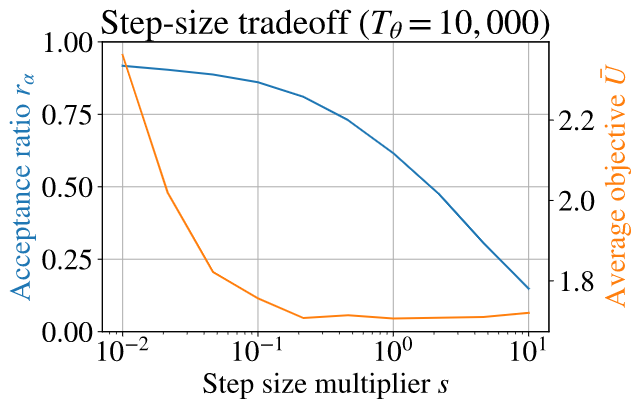
\includegraphics[width=0.6\linewidth]{step-size-tradeoff}
	\caption{Primary school dataset \cite{schools} illustration of step-size tradeoff}
	\label{fig:step-size-tradeoff}
\end{figure}

We see immediately that the acceptance ratio $r_\alpha$ steadily decreases with $s$. This is expected as large jumps for each proposal make it unlikely we stay in a high density region of our target distribution. A low acceptance ratio leads to wasted samples and is obviously undesirable.

Nevertheless, $\bar{U}$ decreases with $s$ indicating shorter burn-in times for larger step-sizes. However, this effect plateaus for $s>0.2$ for this particular dataset. Therefore, we choose $s=0.2$ as our step-size multiplier for the primary school dataset as this yields the best trade-off between $r_\alpha$ and $\bar{U}$. The step-sizes for the other datasets were chosen following the same argument but we do not repeat the process here.

\FloatBarrier
\subsection{Burn-in and thinning}
\label{appdx:burn-in-thinning}

%As with any MCMC method, we must deal with the issues presented by burn-in and thinning.
When sampling from the $b$ and $\theta$-chains described
in Section~\ref{sec:inference}, we respectively generate
$T_b$ and $T_\theta$ samples total.
We discard an initial proportion $\kappa_\star\in(0,1)$ of the samples 
as corresponding to a ``burn-in'' period required for the distribution 
of the chain to reach a distribution close to our target,
and we also ``thin'' the remaining samples to 
obtain a less-dependent version. For $\star\in\{b,\theta\}$,
the remaining sample sets are denoted $\Tcal_\star$
in the notation of Section~\ref{s:ss},
%
\begin{equation}
	\Tcal_\star = \{T_\star \kappa_\star + i \lambda_\star :  
	0 \leq i \leq \lfloor T_\star(1 - \kappa_\star) / \lambda_\star \rfloor \},
\end{equation}
%
where $\lambda_\star$ controls the thinning. The choice of
$\kappa_\star$ can be determined by plotting the log-target (either $S(b^{(t)})$ 
or $U(\theta^{(t)})$ as a function of $t$,
and choosing $\kappa_\star$ to encompass the region where the log-target has 
roughly reached equilibrium. As we do not leverage sample independence,
$\lambda_\star$ can be chosen less rigorously; we often simply
use $\lambda_b=5$ and $\lambda_\theta = 10$.

By way of illustration, we can consider the primary school dataset \cite{schools}. We plot the normalised objective function $U\left( \theta^{(t)} \right) / N$ with respect to MALA iteration on Figure \ref{fig:school-U-orginal} -- using the hyperparameters given in Appendix \ref{appdx:hyperparams}. We see that the chain converges to the modal neighbourhood quickly (within about 2000 iterations of a total 10,000). Nevertheless, we pick $\kappa_\theta=0.4 > 0.2$ to be on the safe-side. $\lambda_\theta=10$ is chosen somewhat arbitrarily as we do not require neighbouring samples to be independent. However, this thinning also has the advantage of speeding up computation of quantities that require an average over all the retained samples -- as $|\Tcal_\theta| < T_\theta$.
%
\begin{figure}[!h]
	\centering
	\begin{subfigure}[t]{0.4\linewidth}
		\centering
		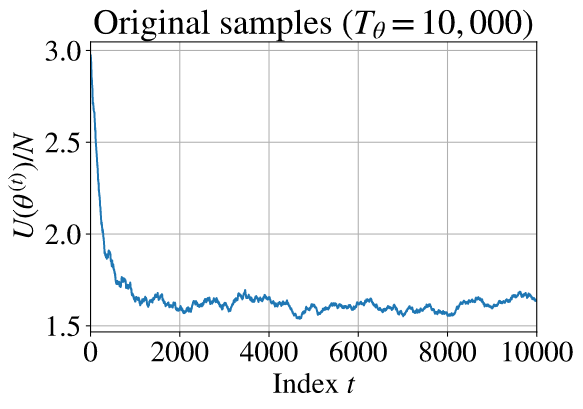
\includegraphics[width=\linewidth]{school-U-original.png}
		\caption{Original samples $t \in [T_\theta]$}
		\label{fig:school-U-orginal}
	\end{subfigure}
	\begin{subfigure}[t]{0.4\linewidth}
		\centering
		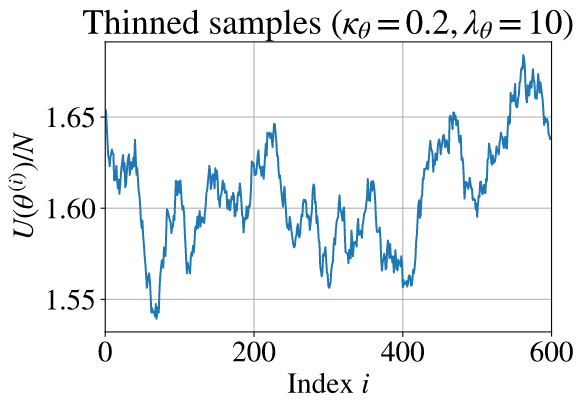
\includegraphics[width=\linewidth]{school-U-thinned.png}
		\caption{Thinned samples $t \in \Tcal_\theta$ indexed by $i$}
		\label{fig:school-U-thinned}
	\end{subfigure}
	\hspace{1cm}
	\caption{Primary school dataset normalised objective function against sample index}
\end{figure}

We plot the retained samples on Figure \ref{fig:school-U-thinned}. $U(\theta^{(i)})/N$ does bounce around a small amount but this is expected as we are sampling from the posterior rather than converging to the MAP solution. There does appear to be variation over a long time-scale but this is acceptable as we do not strictly require sample independence.
\FloatBarrier
\subsection{Initializing the b-chain}

For the purposes of the FFBM model, the number of blocks $B$ is a constant 
which must be specified. If the choice of $B$ is influenced 
by the observed data, then the analysis is no longer ``fully Bayesian''
and belongs to the class of methods referred to as ``empirical Bayes.''
However, as the number of blocks only specifies the coarseness of the 
analysis, it is reasonable to allow it to vary. Indeed, 
\citet{peixoto-determine-B} shows that for a fixed 
average degree the maximum number of detectable blocks scales 
as $O(\sqrt{N})$ where $N$ is the number of vertices.

If $B$ is allowed to vary in the $b$-chain (i.e.,
when new blocks can be created and empty blocks are allowed),
then the chain can be run until a minimum description 
length (MDL) solution is reached. We take the number of non-empty blocks 
in the MDL solution to be our fixed block number $B$ for subsequent analysis. 
Indeed, it is prudent to start the $b$-chain at this MDL solution as then 
the necessary burn-in time can be greatly reduced.

\subsection{Dimensionality discussion}
\label{appdx:dimension}

Many vertex feature often take only one of several discrete values within a set. For example, with the primary school dataset \cite{schools}, a pupil's school-class can take one of 10 values from \{``1A", ``1B", ``2A", ``2B" \dots ``5A", "5B"\}.

It is not immediately obvious how to encode this for the feature-to-block classifier. Although this is technically only a single dimension, we choose to expand the data into a set of 10 binary feature flags all taking values in the set $\Xcal = \{0, 1\}$. Although only one flag will be set at a time it is the simplest method for representing discrete-valued data. The reason we choose $\Xcal=\{0, 1\}$ and not $\Xcal = \{-1, 1\}$ is that the former allows for simpler analysis of the resulting weight values; when a feature $d$ is switched off then $x_{d}=0$ given $\Xcal = \{0, 1\}$, and the feature has no impact on the softmax output. This would not be the case for $\Xcal = \{-1, 1\}$.

Furthermore, it is more intuitive to only model positive relationships. In other words, we prefer to say that this block is comprised of the vertices with feature $d$ turned on rather than this block contains the vertices with feature $d$ switched off. To summarise the approach explicitly, say we have a feature encoding a pupil's gender: \{"male", "female"\}, we represent this as 2 binary feature flags "male": \{0, 1\} and "female": \{0, 1\}. This approach may seem inefficient but it is vital to ensure we can interpret the resulting parameter distributions.

Nevertheless, this dimensionality expansion means that we should not include a bias term in our softmax as then the MAP solution is less peaked and our $\theta$-samples will have higher variance. To illustrate this point we need only look at the form of the softmax activation function with bias vector $\beta$, operating on a vector $x$ which only has one non-zero entry $x_d=1$. Component $j$ of the output is given by:
%
\begin{equation}
	\phi_j(x) = \frac{\exp(w_j^T x + \beta_j)}{\sum_{k \in [B]} \exp(w_k^T x + \beta_k)} = 
	\frac{\exp(w_{jd} + \beta_j)}{\sum_{k \in [B]} \exp({w_{kd} + \beta_k})}.
	\label{eqn:softmax-bias}
\end{equation}
%
The term $w_{kd} + \beta_k$ is effectively the new weight for component $k$ as these two terms will always appear together. The bias term $\beta_k$ is therefore an unnecessary extra degree of freedom. To illustrate this point, we set $\beta_k=\beta_0$ for all $j$. If this is the case then equation \ref{eqn:softmax-bias} can be simplified to:
%
\begin{equation}
	\phi_j(x) = \frac{\exp(\beta_0) \cdot \exp(w_{jd})}{\sum_{k \in [B]} \exp(\beta_0) \cdot \exp(w_{kd})}
	= \frac{\exp(w_{jd})}{\sum_{k \in [B]} \exp(w_{kd})}
\end{equation}
%
This expression is independent of $\beta_0$ and so it is free to vary. This is not the whole picture as we also have the prior which introduces a regularisation term which favours weights closer to 0. This ensures the MAP solution is unique. Nevertheless, for mutually exclusive binary feature flags, the bias term does not add to the expressiveness of the model and only serves to complicate analysis. We therefore remove the bias term from the softmax.

Even for data comprised of several feature-classes each expanded into flags (e.g. school class and gender) we prefer to discard the bias term. The bias term only serves to decrease the objective function by leveraging information about the size of each detected block and not feature information. We do not wish to be overly confident in our block predictions when such predictions are influenced by block size and not feature information. Indeed, the approach was initially developed with a bias term but we found its removal yielded more reliable and reproducible results.

\subsection{Hypothesis test on feature weights}
\label{appdx:hyp-test}

We are given samples $\{\theta^{(t)}\}_{t \in \Tcal_\theta} \sim p(\theta | A, X)$ and wish to determine the statistical significance of the weights. We adopt matrix notation for simplicity by representing $\theta$ with the matrix $B \times D$ matrix of feature weights $W$. The question is to determine the significance of a particular feature $d$ by examining the value of $W_{id}$ for all the values $i \in [B]$. We know that the posterior is proportional to the prior multiplied by the likelihood,
%
\begin{equation}
	p(\theta|A, X) \propto p(\theta) \cdot p(A | \theta, X),
\end{equation}
%
assuming that the feature matrix $X$ is already given. The prior term can be evaluated but the likelihood is intractable. The closest we can get is through a Monte-Carlo integration over $b$,
%
\begin{align}
	p(A | \theta, X) &= \sum_{b \in [B]^N} p(A, b | \theta, X) \nonumber \\
	&= \sum_{b \in [B]^N} p(A | b, \theta, X) \cdot p(b | \theta, X) \nonumber \\
	&= \sum_{b \in [B]^N} p(A | b) \cdot p(b | \theta, X) \nonumber \\
	&\approx \sum_{i} p\left( A | b^{(i)} \right) \quad \textrm{with} \quad b^{(i)} \sim p(b| \theta, X).
	\label{eqn:mc-likelihood}
\end{align}
%
This could be implemented for a single value of $\theta$ but such a form cannot be used to characterise the overall form of the posterior. Nevertheless, the form in~(\ref{eqn:mc-likelihood}) highlights something interesting. The likelihood is peaked around areas of $\theta$ that generate a partition $b$ that is highly likely in the SBM sense -- high $p(A|b)$. This provides the motivation for using the Laplace approximation for modelling the posterior $p(\theta | A, X) \approx p(\theta; \hat{\mu}, \hat{\Sigma})$; we use a multivariate Gaussian to approximate the posterior. Indeed, the Laplace approximation is often used for modelling the posterior in logistic classification \cite{laplace}. This approximation is not exact but it motivates the derivation of the dimensionality reduction technique we construct by analogy with hypothesis testing. Marginalising over the other elements, the posterior for each element of the weight matrix $W$ can be approximated by,
%
\begin{equation}
	p(W_{ij}|A, X) \approx \Gaussian(W_{ij}|\hat{\mu}_{ij}, \hat{\sigma}_{ij}^2).
\end{equation}
%
Where we have used the set of samples for $W$ drawn according to the exact posterior, to calculate unbiased estimates for the mean and standard deviation:
%
\begin{equation}
	\hat{\mu}_{ij} \coloneqq \frac{1}{|\Tcal_\theta|} \sum_{t \in \Tcal_\theta} W_{ij}^{(t)} \qquad \textrm{and} \qquad
	\hat{\sigma}_{ij}^2 \coloneqq \frac{1}{|\Tcal_\theta|} \sum_{t \in \Tcal_\theta} \left( W_{ij}^{(t)} - \hat{\mu}_{ij} \right)^2.
\end{equation}
%
This approximation is not exact but we can show it is accurate empirically. Indeed, if we run the primary school experiment with hyper-parameters given in Appendix \ref{appdx:hyperparams}, we can then plot histograms of the collected $W$-samples and compare these to the Laplace approximation. The results are given on Figure \ref{fig:school-histogram}. Even though the Laplace approximation is not exact, it is remarkably reliable. 

\begin{figure}[!h]
	\centering
	\begin{subfigure}[t]{0.32\linewidth}
		\centering
		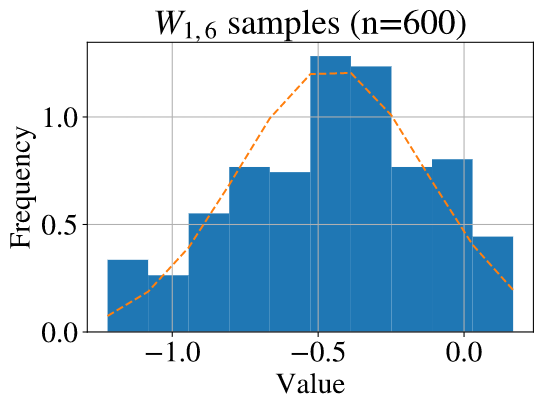
\includegraphics[width=\linewidth]{school-sample-histogram-16.png}
		\caption{Weight for block 1, class 3B}
	\end{subfigure}
	\hfill
	\begin{subfigure}[t]{0.32\linewidth}
		\centering
		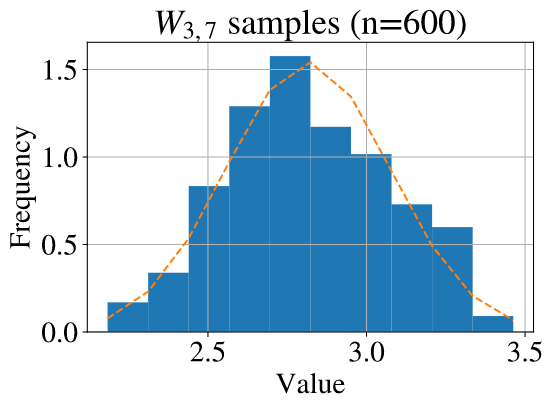
\includegraphics[width=\linewidth]{school-sample-histogram-37.png}
		\caption{Weight for block 3, class 4A}
	\end{subfigure}
	\hfill
	\begin{subfigure}[t]{0.32\linewidth}
		\centering
		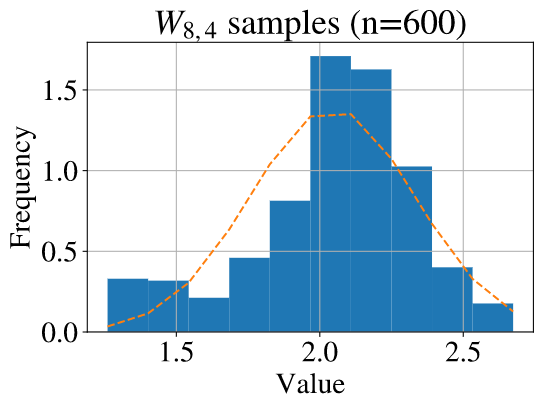
\includegraphics[width=\linewidth]{school-sample-histogram-84.png}
		\caption{Weight for block 8, class 2B}
	\end{subfigure}
	
	\caption{Histograms of sampled weights for the primary school experiment \cite{schools}. Dotted line is the applied Laplace approximation.}
	\label{fig:school-histogram}
\end{figure}

Using the approximation, we wish to construct a test to determine whether a particular weight value has $|W_{ij}| > c$ with high probability, where $c>0$. More specifically, we wish to decide between:
%
\begin{equation}
	\begin{aligned}
		H_0&: |W_{ij}| \leq c \\
		H_1&: |W_{ij}| > c
	\end{aligned}
\end{equation}
%
We can consider the probabilities $p(W_{ij} > c)$ and $p(W_{ij} < c)$ separately. Starting with $p(W_{ij} > c)$, we write this as,
%
\begin{align*}
	p(W_{ij} > c) &= p\left(Z > \frac{c - \hat{\mu}_{ij}}{\hat{\sigma}_{ij}}\right) \\
	&= p\left(-Z < \frac{\hat{\mu}_{ij} - c}{\hat{\sigma}_{ij}}\right)\\
	&= \Phi\left(\frac{\hat{\mu}_{ij} - c}{\hat{\sigma}_{ij}}\right),
\end{align*}
%
where $Z \sim \Gaussian(0,1)$ and $\Phi(\cdot)$ is the standard Gaussian cumulative density function. We introduce the variable $k$ to control the degree of significance of the result. Enforcing $k$ to be less than the argument of $\Phi$ gives us that: 
%
\begin{equation*}
	\hat{\mu}_{ij} - k \hat{\sigma}_{ij} > c.
\end{equation*}
%
As $\Phi(\cdot)$ is monotonically increasing, this yields the following:
%
\begin{equation}
	p(W_{ij} > c) > \Phi(k) \iff \hat{\mu}_{ij} - k \hat{\sigma}_{ij} > c.
	\label{eqn:hyp-test-positive}
\end{equation}
%
A similar argument can be made to show that:
%
\begin{equation}
	p(W_{ij} < -c) > \Phi(k) \iff \hat{\mu}_{ij} + k \hat{\sigma}_{ij} < -c.
	\label{eqn:hyp-test-negative}
\end{equation}
%
Clearly equations \ref{eqn:hyp-test-positive} and \ref{eqn:hyp-test-negative} cannot both hold simultaneously as $c, \hat{\sigma}_{ij}, k>0$. Nevertheless, a necessary and sufficient condition for one of them to hold is:
%
\begin{equation}
	(\hat{\mu}_{ij} - k \hat{\sigma}_{ij}, \hat{\mu}_{ij} + k \hat{\sigma}_{ij}) \cap (-c, +c) = \emptyset
	\label{eqn:hyp-test-empty}
\end{equation}
%
This is equivalent to saying that $\hat{\mu}_{ij}$ is at least $k$ standard deviations away from the range $(-c, c)$. We choose to reject the null hypothesis $H_0$ if and only if equation \ref{eqn:hyp-test-empty} holds. We can say with probability greater than or equal to $\Phi(k)$ that either $W_{ij} < -c$ or $W_{ij} > c$ thus rejecting the null $H_0: |W_{ij}| \leq c$.

Note that we choose to accept $H_0$ even in the case that the combined probabilities of $p(W_{ij} < -c) + p(W_{ij} > c) > \Phi(k)$, if equation \ref{eqn:hyp-test-empty} is not satisfied. This is because we wish to apply this for dimensionality reduction purposes. We only want to keep weights for which we have a confident prediction outside the range $(-c, c)$ not those that succeed by summing the two extremes of their distribution. Note that this case is very rare empirically but it nonetheless must be specified.